%\vspace{-.15in}
\section{Methods}
\label{sec:method}

\begin{comment}
\begin{itemize}
    \item Computing field lines through the XGC mesh.
    \item Equation for RK4
    \item Describe XGC mesh
    \item Describe the algorithm
    \item Parallelization with \vtkm.
    \item Convenient to use cylindrical coordinates for tracing.
    \item Evaluation of magnetic fields
    \begin{itemize}
        \item XGC grid (2D triangle grid, N planes)
        \item XGC formulation of magnetic fields
    \end{itemize}
\end{itemize}
\end{comment}

Computing the \poincare map consists of two basic steps. First, compute field lines originating from each seed location. Second, intersect the fieldlines with the \poincare section.
Fieldlines, or streamlines, are generated by computing the trajectory of a massless particle through a  vector field. 
This is a classic initial value problem, $\frac{dy}{dt} = f(t,y)$, where $y(t_0) = y_0$. Here, $y_0$ is the (seed) location at time $t_0$, and $f(t,y)$ is the vector field. For streamline computation, a common method for computing the trajectory of the particle ($y(t)$), is using the $4^{th}$ order Runge-Kutta iterative method~\cite{PresTeukVettFlan92}. For a given step size $h > 0$, positions along the trajectory ($y_i)$ can be computed by:
%\vspace{-.1in}
\begin{align}
    y_{n+1} = y_n  + \frac{h}{6} (k_1 + 2k_2 + 2k_3 + k_4)
    \label{eq:RK4}
\end{align}
\vspace{-.1in}
where
%\vspace{-.1in}
\begin{align*}
k_1 &= f(t_n,\quad y_n) \\
k_2 &= f(t_n+\frac{h}{2},\ y_n + h\frac{k_1}{2}) \\
k_3 &= f(t_n+\frac{h}{2},\: y_n + h\frac{k_2}{2}) \\
k_4 &= f(t_n+\frac{h}{2},\; y_n + hk_3)
\end{align*}
\vspace{-.3in}


\begin{figure}[htb]
  \centering
  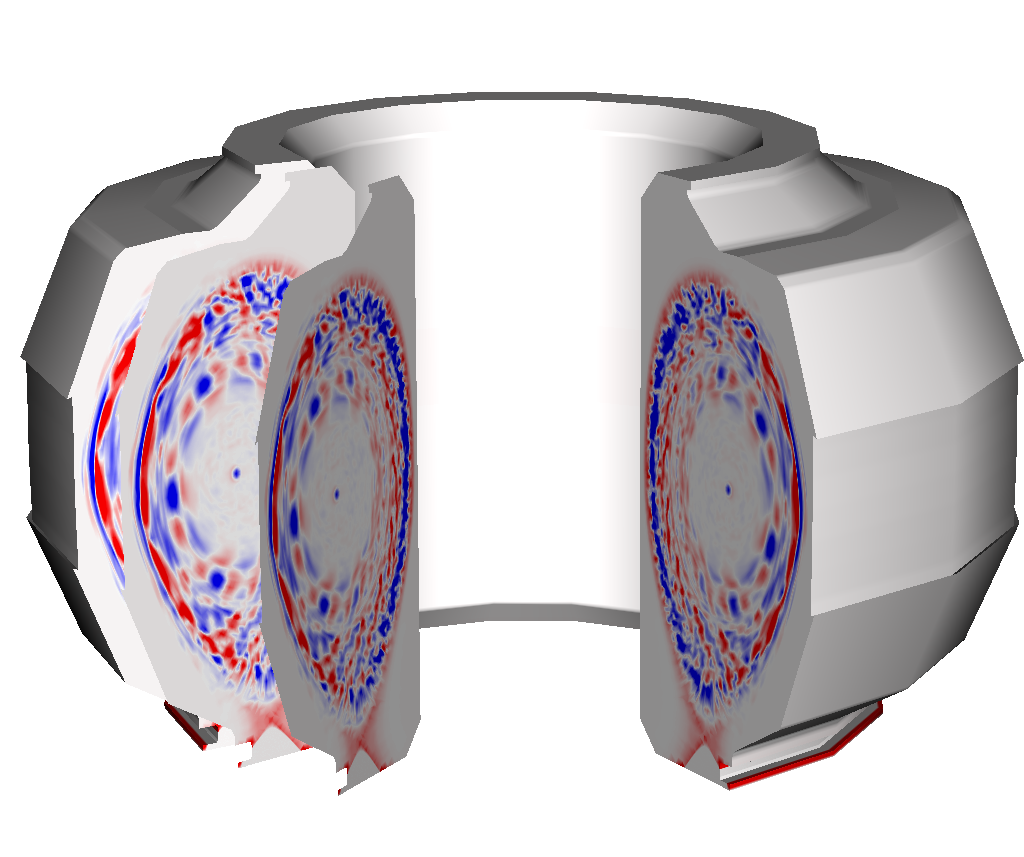
\includegraphics[height=1.5in]{figures/xgc2.png}
\vspace{-.15in}
  \caption{Example of an XGC mesh that has been clipped to show the interior. 2D planes are equally spaced around the central axis of the tokamak. Two planes are shown in the clipped region to illustrate the semi-unstructured nature of the mesh.}
  \label{fig:xgc_mesh}
\end{figure}

The key requirement of the RK4 method is to be able to evaluate $f(t,y)$ (i.e., the magnetic field) at each point within the domain.

The XGC code uses a semi-unstructured mesh to represent the physics of the plasma. Fundamentally, the mesh is cylindrical with periodic boundary conditions along the cylinder's axis. The mesh is structured along the axis of the cylinder and each toroidal cross-section is a 2D unstructured triangular mesh.
The cross-section is rotated around the central axis to create the 3D mesh (see  Figure~\ref{fig:xgc_mesh}).
The mesh consists of wedge elements that are formed from pairs of triangles from adjacent planar cross sections.


\subsection{\poincare Algorithm}
\label{sec:algorithm}
\algnewcommand\algorithmicforeach{\textbf{for each:}}
\algnewcommand\ForEach{\item[ \algorithmicforeach]}

\begin{algorithm}
\caption{Algorithm for computing a \poincare map.}
\label{alg:poinc}

\begin{algorithmic}[1]
\State \textbf{/* Initialization */}
\State $P$ = \poincare section \label{alg:poinc:init0}
\State $S$ = Input seed locations
\State $Max_p$ = Maximum number of punctures
\State $Result = Empty$ \label{alg:poinc:init1}
\State 
\ForAll{$s$ in $S$} \label{alg:poinc:forLoop0}
  \State \textbf{/* Compute the \poincare map for the field line at $s$ */}
  \State $n = 0$ %\bf{ /* Number of punctures for seed */}
  \State $p_0 = s$ 
  \State
  \State \textbf{/* Iterate until max number of punctures computed */}
  \While{$n < Max_p$}  \label{alg:poinc:whileLoop0}
    \State $p_1 = $ RK4Solve($p_0$)
    \State $L = $ line segment from $p_0$ to $p_1$
    \If{$L$ intersects $P$} \label{alg:poinc:intersect_check}
      \State Add intersection of $L$ and $P$ to $Result$
      \State $n = n + 1$
     \EndIf
    \State $p_0 = p_1$
   \EndWhile  \label{alg:poinc:whileLoop1}
\EndFor   \label{alg:poinc:forLoop1}

\end{algorithmic}
\end{algorithm}


Algorithm~\ref{alg:poinc} contains pseudocode for computing the \poincare map.
Initialization consists of specifying the initial seed locations, defining the \poincare section (i.e., 2D plane), and the maximum number of punctures to compute as well as initializing a structure to store punctures (Lines \ref{alg:poinc:init0} - \ref{alg:poinc:init1}).
For each seed location $s$ (Line~\ref{alg:poinc:forLoop0}), the fieldline is iteratively computed using a RK4 solver. At each iteration of the solver, the line segment between the current location and the previous location is checked against the \poincare section to determine if an intersection occurred (Line~\ref{alg:poinc:intersect_check}).
If so, the intersection point is added to the result.
This process continues until the maximum number of punctures occurs, or the particle terminates. For brevity, the code to check for particle termination is not shown in the code listing.

\subsection{Implementation in \vtkm}
\vtkm uses a data parallel abstraction to achieve high performance on many-core devices~\cite{MCD3:2021}.
Given a vector of data, \vtkm will apply a function to each element of the array. These functions often come in the form of ``functors,'' which is an object that can be called like an ordinary function. 
The input data to the \vtkm implementation of the \poincare algorithm is an array of initial particle positions. 
The functor object is initialized with the \poincare section, RK4 step size and the maximum number of punctures.
The execution portion of the functor consists of lines~\ref{alg:poinc:forLoop0}-~\ref{alg:poinc:forLoop1} in Algorithm~\ref{alg:poinc}.
At runtime, each input particle and the functor are mapped to a thread and executed on the specified device, effectively making the for loop parallel.

\begin{comment}
\begin{figure}[htb]
  \centering
  
\includegraphics[height=1in]{figures/Ed}
  
\includegraphics[height=1in]{figures/Ed}

  \caption{Projection of $(x,y,\phi$) onto 2D. Consider tossing this figure.}
  \label{fig:project2d}
\end{figure}
\end{comment}

The bottleneck of the algorithm is not the arithmetic used to compute Equation~\ref{eq:RK4} for the RK4 solution but rather the field evaluation to get the numbers to plug into the equation.
At each iteration of the algorithm, the cell containing the current location of the point must be determined. Because the mesh is unstructured, this requires a cell search. This search can be optimized by taking advantage of the toroidal symmetry of the mesh.
Using this symmetry, the point can be specified by $(x,y,\phi)$, where $x$ and $y$ are coordinates of the 2D cross-section and $\phi$ is the angle around the torus. The point can be easily projected onto the 2D cross section by setting $\phi = 0$ (i.e., $(x,y,0)$).
The cell-finding operation is now reduced to two dimensions.

To accelerate the cell-finding operation for unstructured grids, \vtkm provides two different acceleration structures. The first uses two levels of structured grids~\cite{Kalojanov2011}. The first level is a coarse grid of bins that covers the spatial extents of the data. Each bin within the first level contains a finer grid where the number of bins is proportional to the number of cells contained in the first level grid. Each bin in the fine-level grids contains a list of unstructured cells that are contained.
The second acceleration structure is much simpler. It uses a single fine-structured grid. As before, each bin contains a list of the unstructured cells that are contained.
For each method, the 2D cross-section mesh is passed in, and the acceleration structure is built. The acceleration structure is passed into the \vtkm functor to be used for field evaluations.

The major costs for either structure are the time to retrieve the appropriate bin and the time to search through the cells in the bin.
The advantage of the simpler uniform bin approach is that the appropriate bin can be found with a single lookup rather than the two-part lookup of the two-level grid.
However, the two-level grid avoids bins containing large numbers of unstructured cells when the unstructured cells are unevenly distributed.

In either case, whenever the algorithm looks up a cell, it remembers both the unstructured cell found and the bin containing it.
Subsequent field evaluations will be nearby and are often in the same cell or a nearby one.
Before searching for a bin, the algorithm first checks the saved unstructured cell for containment and then the saved bin.

\subsection{Field Evaluation}
For many applications, the vector field values are defined at the vertices of each cell. Evaluation at a location within the cell interpolates the values at each of the vertices. However, the magnetic field in XGC is much more complicated. Because calculating fieldlines contains many iterative steps, accuracy is paramount as small errors can rapidly grow and produce incorrect results.

In XGC, the magnetic field vector consists of an axisymmetric (i.e., defined at the cross-sectional plane and constant along the cylindrical axis) background field, $\boldsymbol{B}_0$ and a non-axisymmetric perturbation, $\delta\boldsymbol{B}$.
For a particle located at $(x,y,\phi)$, the magnetic field is sum of the background field and the perturbation: $\boldsymbol_{B}_0(x,y) + \delta\boldsymbol{B}(x,y,\phi)$.
The background field, $\boldsymbol{B}_0$,  is evaluated using cubic spline interpolation using the $2D$ coordinates $(x,y)$.
The perturbation is represented as the component of the magnetic vector potential parallel to the background magnetic field $A_\parallel(x,y,\varphi)$, on a set of $N_\varphi$ planar, unstructured triangle meshes, where $N_\varphi$ is the toroidal resolution of the XGC simulation.  In practice, for large runs, $N_\varphi$ is between 32 and 64, depending on the physics being studied. The corresponding perturbed magnetic field is $\delta\boldsymbol{B}=\nabla\times(A_\parallel \boldsymbol{B}_0/|\boldsymbol{B}_0|)$.
For interpolation of data between planes, the magnetic vector potential and its derivatives are interpolated linearly along the magnetic field line through the position of the particle. This requires interpolation on two cross-sectional planes, which is also linear. To minimize interpolation errors, the mesh in XGC is approximately aligned with the magnetic field such that a field line starting on a vertex on one plane maps along $\boldsymbol{B}_0$ to a position at or very close to a mesh vertex on the adjacent plane. For a more detailed explanation is given in~\cite{moritaka_2019, Hariri2013, HAGER2016644}.

Accurately calculating the non-axisymmetric perturbation of the magnetic field, ($\delta\boldsymbol{B}$), was the most challenging part of the collaboration.
The XGC implementation of the \poincare\ tool is embedded within the XGC simulation code. The \poincare\ tool is run by using an input deck for the simulation that specifies how to configure and run the analysis. As such, the code for performing a full simulation and \poincare\ analysis share some non-trivial overlap that must be carefully separated. Further, given that XGC is written in Fortran, and \vtkm is written in C++, the code separation must be done carefully and is easy to get wrong. We instrumented the XGC code with debug logs to check the calculation of key quantities in the derivation of the magnetic field at each step of a point along a field line. The coordinates of individual field lines were also saved so that they could be compared (both visually and textually) to the coordinates generated by the \vtkm implementation. When differences in coordinates were detected, we were able to compare, step by step, the computation of the different values associated with the calculation of $\boldsymbol{B}_0$ and $\delta\boldsymbol{B}$ in both codes and determine where the errors occurred. Once these were identified and fixed, we ran both the XGC and \vtkm implementations of the code over many different seeding scenarios and physics parameters and compared the resulting \poincare plots to ensure they were identical.

In an attempt to optimize the calculation of the perturbed magnet field, we pre-computed $\boldsymbol_{B}_0(x,y) + \delta\boldsymbol{B}(x,y,\phi)$ at each vertex in the $3D$ mesh to avoid the complexity of the field evaluation at every RK4 iteration. However, the effects of linear interpolation of the values within the 3D elements of the mesh over a large number of iterations resulted in errors that compounded over thousands of RK4 steps and produced significantly inaccurate results. In the end, this optimization had to be abandoned.


\begin{comment}
\begin{itemize}
  \item Magnetic field vector consists of an axisymmetric (i.e., constant in the cylindrical angle $\varphi$) background and a non-axisymmetric perturbation
  \item The background field $\boldsymbol{B}_0$ is fully described by two functions, $\psi(R,Z)$, where $R$ and $Z$ are cylindrical coordinates, and $F(\psi)$. (Can add the formula, if necessary.)
  \item The background field is evaluated using cubic spline interpolation using only the marker position $(R,Z)$.
  \item The perturbation is represented as the component of the magnetic vector potential parallel to the background magnetic field, $A_\parallel(R,Z,\varphi)$, on a set of $N_\varphi$ planar, unstructured triangle meshes, where $N_\varphi$ is the toroidal resolution of the XGC simulation. 
  \item The corresponding perturbed magnetic field is $\delta\boldsymbol{B}=\nabla\times(A_\parallel \boldsymbol{B}_0/|\boldsymbol{B}_0|$.
  \item For interpolation of data between planes, the magnetic vector potential and its derivatives are interpolated linearly along the magnetic field line through the position of a marker. This requires interpolation on two $(R,Z)$ planes, which is also linear.
  \item To minimize interpolation errors, the mesh in XGC is approximately aligned with the magnetic field such that a field line starting on a vertex on one plane maps along $\boldsymbol{B}_0$ to a position at or very close to a mesh vertex on the adjacent plane.
  
\end{itemize}
\end{comment}
 







